\chapter{A kártyák}

A játék egyik ha nem legfontosabb eleme a kártyák. Összesen a játék 44 egyedi kártyát tartalmaz. Karakter klassonként 5 kártyát és 4 klass függetlent. Fontos a kártyák színe ami a klasshoz való tartozásukat szimbolizálja. Ezek a színek a :\\\
     Warrior - Piros és árnyalatai \\\
     Ranger - Barna és árnyalatai\\\
     Mage - Kék és árnyalatai\\\
     Paladin - Sárga és árnyalatai\\\
     Druid - Zöld és árnyalatai\\\
     Ninja - Lila és árnyalatai\\\
     Necromancer - Sötét Lila és Szürkék\\\
     Alchemist - Rózsaszín és árnyalatai\\\

\section{Kártya Típusok}
A játék 5 nagy kártya típussal operál: Felszerelés, Varázslat, Aréna Effektus, Idézett lény és Token. Ezek más más tulajdonságokkal bírnak és máshogy működnek.
\begin{itemize}
    \item Felszerelés:\\
    Álatlánosan a játékosnak ad fizikai vagy mágikus bónusz sebzést. Ezek a játékos karakterétől jobbra és barra lévő helyekre lehet lehelyezni.
    \item Varázslat:\\\
    Ezek a kártyák kijátszáskor valamit csinálnak. Ez lehet sebzés, gyógyítás, kártyahúzás stb.
    \item Aréna Effektus:\\\
    Passzív effektekkel bírnak melyek vagy a kör elején vagy a végén akitválódnak.
    \item Idézett lények:\\\
    Ezek a Felszereléshez hasonlőan működnek de a sebzés bónuszon túl azzal a tulajdonsággal bírnak hogy együtt támadnak a játékossal.
    \item Token:\\\
    A Tokenek a Varázslatokhoz hasonlóak annyi külömbséggel hogy egyszehasználatosak, kártyák generálják őket, a sebzésük nem függ a játékos fizikai és vagy mágikus sebzés bónuszától illetve nem kerülnek semmilyen pontba. 
\end{itemize}

\section{Kártya felépítése}
\subsection{Proof of concept}
\begin{itemize}
    \item A bal felső sarokban látható a kártya ára. A zöld gömb az akció pontot jelenti, a sárga háromszög pedig a reakciópontot. A mennyiség pedig hogy mennyi pontba kerül a kártya.
    \item Középen található a kártya neve.
    \item A név felett található egy kis rajz a kártyához illetve a keret. A keret határozza meg illetve közli a játékossal hogy milyen típusú kártyáról van szó. Hatszög szerű = felszerelés, ovális = aréna effektus, stb.
    \item A név alatt található a kártya leírás.
    \item A bal alsó sarokban található a sebzés értéke a kártyának.
\end{itemize}

\subsection{Place Holder}
\begin{itemize}
    \item A bal felső sarokban látható a kártya ára. Először a mennyiség szerepel majd a pont típusa
    \item Középen található a kártya neve.
    \item A név felett található a kártya típusa. Ezek lehetnek: Varázslat, Felszerelés, Aréna Effeckt, Idézett lény, Token.
    \item A név alatt található a kártya leírás.
    \item A bal alsó sarokban található a sebzés értéke a kártyának.
\end{itemize}

A kártyák a jövőben hasonlóan néznének ki a Sword számára elkészült rajz.

\begin{figure}[h]
        \centering
        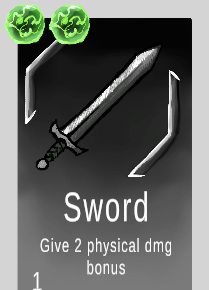
\includegraphics[width=140px,keepaspectratio]{images/SwordPic.png}
        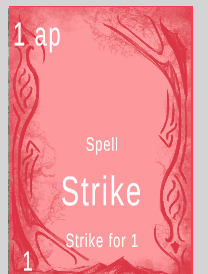
\includegraphics[width=140px,keepaspectratio]{images/Strike.png}
        \label{POC}
        \caption { Koncepció a tényleges kártyákról és a place holder kártya}
    \hspace{1em}
\end{figure}

\section{Általános}

\begin{itemize}
    \item Strike - Varázslat\\\
    - Ára: 1 akció pont \\\
    A kártya 1 + fizikai sebzés bónusz sebzést okoz az ellenfélnek.
    \item Defend - Varázslat\\\
    - Ára: 1 reakció pont \\\
    A játékos 2 pajzspontot kap.
    \item Draw - Varázslat\\\
    - Ára: 2 reakció pont \\\
    A játékos húz egy kártyát.
    \item Sword - Felszerelés\\\
    - Ára: 2 akció pont \\\
    Egy szimpla kard  ami 2 bónusz fizikai sebzést ad.
\end{itemize}

\section{Warrior}
\begin{itemize}
    \item Blood Thirster - Felszerelés:\\\
    - Ára: 2 akció pont \\\
    A kártya plusz 1 fizikai sebzés bónuszt kap az összes ebben a körben az összes kijátszás előtt kijátszott Strike ért. Ebbe bele tartozik a Fury Strike (plus annyi Strike ahányszor a kártya aktiválódott), Double Strike (plus 2) és a Throw Weapon is. 
    \item Flesh Ripper - Felszerelés:\\\
    - Ára: 3 akció pont \\\
    Ha a játékos Strike-ot játszik ki akkor a támadás előtt elpusztítja az ellenfél 2 pajzspontját majd utána támad.
    \item Double Strike - Varázslat\\\
    - Ára: 2 akció pont \\\
    A játékos kétszer kijátsza a Strike-ot.
    \item Fury Strikes - Varázslat\\\
    - Ára: x akció pont \\\
    A játékos annyi Strike kártyát játszik ki ammenyi elérhető akció pontja van. Mindegy egyes kijátszott Strike után elkült 1 akció pontot.
    \item Battle Rage - Varázslat\\\
    - Ára: 1 reakció pont \\\
    A játékos ebben a körben kap 2 bónusz fizikia és mágikus sebzést.
\end{itemize}

\clearpage
\section{Ranger}
\begin{itemize}
    \item Ranger Bow - Felszerelés:\\\
    - Ára: 1 akció pont \\\
    A kártya plus 1 fizikai sebzés bónuszt ad.
    \item Crossbow - Felszerelés:\\\
    - Ára: 3 akció pont \\\
    A kártya plus 3 fizikai sebzés bónuszt ad illetve minden kör elején ad egy extra akció pontot..
    \item Aroow Volley - Varázslat:\\\
    - Ára: 2 akció pont \\\
    A kártya kilő 4 + a fizikai és mágikus bónusz sebzés darab nyilat melyek mind 1 sebzést okoznak. 
    \item Wind Sweapt Hills - Aréna Effektus:\\\
    - Ára: 2 reakció pont \\\
    Ha a kártya aktív a játékos a köre elején egy extra lapot húz fel.
    \item Hunters Trap - Aréna Effektus:\\\
    - Ára: 2 akció pont \\\
    Ha az ellenfél megtámadja a játékost akkor az ellenfél elszenved 1 sebzést.
\end{itemize}

\section{Mage}
\begin{itemize}
    \item Sorcefull Staff - Felszerelés:\\\
    - Ára: 2 akció pont \\\
    A kártya plus 3 mágikus sebzés bónuszt ad. Ha a felszerelés használva van akkor a Strike kártyák sebzéséhez hozzá adódik a játékos mágikus sebzés bónusza is. 
    \item Arcane Spellbook - Felszerelés:\\\
    - Ára: 2 reakció pont \\\
    A kártya plus 1 mágikus sebzés bónuszt ad. Amíg a kártya a táblán van a játékos minden egyes kijátszott vatázslat után felhúz egy kártyát.
    \item Arcane Spike - Varázslat:\\\
    - Ára: 1 akció pont \\\
    A kártya kioszt 1 sebzést 3 + bónusz mágikus sebzés szer.
    \item Magic Missle - Varázslat:\\\
    - Ára: 3 akció pont \\\
    A játékos előkészít egy hatalmas mágikus csapást. Ez a támadás a játékos bónusz mágikus sebzésének három szorosát sebzi az ellenfélbe.
    \item The Storm - Aréna Effektus:\\\
    - Ára: 2 reakció pont \\\
    Ha ez a kártya a pályán van akkor a játékos általi támadások (akár levédi az ellenfél pajzsa akár nem) 1 sebzést okoznak azonnal az ellenfél életpontjainak.
\end{itemize}

\section{Paladin}
\begin{itemize}
    \item Paladin Shield - Felszerelés:\\\
    - Ára: 2 reakció pont \\\
    A kör elején a játékos kap egy pajzs pontot.
    \item Provoke - Varázslat:\\\
    - Ára: 1 akció pont \\\
    Kijátszáskor a játékos egy pajzs pontot kap illetve húz egy kártyát.
    \item Holy Block - Varázslat:\\\
    - Ára: 2 reakció pont \\\
    Amikor a játékos kijátsza ezt a kártyát azonnal 5 pajzs pontot kap. Ezen felül 2 mágikus sebzés bónuszt kap erre a körre.
    \item Shield Throw - Varázslat:\\\
    - Ára: 2 akció pont \\\
    A játékos a pájzsát használva az offenzívára tör. Az ellenfél annyit sebződik amennyi pajzsa van a játékosnak.
    \item Mountain Stance - Aréna Effektus:\\\
    - Ára: 3 reakció pont \\\
    Ha a játékos több sebzést ka mint amennyi pajzs pontja van akkor kap 1 pajzs pontot.
\end{itemize}

\section{Druid}
\begin{itemize}
    \item Druid Staff - Felszerelés:\\\
    - Ára: 2 akció pont \\\
    A kártya plus 3 mágikus sebzés bónuszt ad. A kör elején gyógyítja a játékost 1 + mágikus sebzés búnusz mennyiséggel.
    \item Visous Veins - Aréna Effektus:\\\
    - Ára: 2 akció pont \\\
    Agresszív gyökerek körbeveszik az ellenfelet. Az ellenfél a köre elején elveszít egy akció pontot illetve a gyökerek elpusztítjék2 pajzs pontját.
    \item Forest Of Favours - Aréna Effektus:\\\
    - Ára: 3 reakció pont \\\
    Ha a kártya a pályán van a játékos a köre elején gyógyul 1 + mágikus sebzés búnusz mennyiséget és kap egy extra akciópontot.
    \item Woddland Mending - Varázslat:\\\
    - Ára: 2 akció pont \\\
    A játékos gyógyul 3 + mágikus sebzés búnusz mennyiséget míg az ellenfél elszenved ugyan ennyit.
    \item Meditation - Varázslat:\\\
    - Ára: 3 akció pont \\\
    A játékos felhúz egy kártyát. A következő köben felerősíti magát. A Kört 2 extra akció pontal kezdi illetve kap 3 mágikus sebzés bónusz erre a körre. 
\end{itemize}

\section{Ninja}
\begin{itemize}
    \item Kunai - Felszerelés:\\\
    - Ára: 1 akció pont \\\
    A kártya plus 1 fizikai sebzés bónuszt ad. A kör elején generál egy Dagger Token kártyát.
    \item Kyoketsu-smoge - Felszerelés:\\\
    - Ára: 3 akció pont \\\
     A kártya plus 3 fizikai sebzés bónuszt ad. A Kör végén a körben kijátszott 
     Strike-ok + 1-el egyenlő mennyiségű sebzést okoz az ellenfélnek.
    \item Pocket Daggers - Varázslat:\\\
    - Ára: 1 akció pont \\\
    Generál 2 Dagger kártyát a játékos kezébe.
    \item Sharp Daggers - Varázslat:\\\
    - Ára: 3 akció pont \\\
    Generál 4 Dagger Kártyát a játékos kezébe. Ebben a körben a Dagger kártyák sebzése 1-ről 3-ra nő
    \item Weapon Throw - Felszerelés:\\\
    - Ára: 0 akció pont \\\
    A Játékos eldobja az egy felszerelését és ezzel Strike-ol egyet.
    \item Dagger - Token:\\\
    - Ára: 0 akció pont \\\
    A kártya kijátszáskor 1-et sebez az ellenfélbe.
\end{itemize}

\section{Nercomancer}
\begin{itemize}
    \item Bob - Idézett lény:\\\
    - Ára: 3 akció pont \\\
    Bob egy feltámasztott csontváz katona, 3 fizikai sebzés bónuszt ad és ha a játékos Strike kártyát játszik ki akkor megtámadja az ellenfelet és 2 sebzést okoz.
    \item Harly - Idézett lény:\\\
    - Ára: 3 reakció pont \\\
    Harly egy feltámasztott csontváz Mágus, 3 mágikus sebzés bónuszt ad és ha a játékos Strike kártyát játszik ki akkor megtámadja az ellenfelet és 2 sebzést okos.
    \item Decaying Touch - Varázslat:\\\
    - Ára: 2 akció pont \\\
    A játékos 3 + mágikus sebzés bónus sebzést okoz az ellenfelénel és ezt a sebzést vissza gyógyítja magán.
    \item Forbidden Knowledge - Varázslat:\\\
    - Ára: 1 reakció pont \\\
    A játékos feláldoz 2 élet pontot és ezért felhúz 2 lapot.
    \item The Graveyard - Aréna Effektus:\\\
    - Ára: 1 reakció pont \\\
    A játékos a körei végén kap 2 pajzs pontot.
\end{itemize}

\section{Alchemist}
\begin{itemize}
    \item Alchemists gloves - Felszerelés:\\\
    - Ára: 3 reakció pont \\\
    A kör elején kreál egy potiont a játékos kezébe. Az első kijátszott Potion kártyáról csinál egy másolatot a játékos kezébe.
    \item Potion launcher - Felszerelés:\\\
    - Ára: 3 akció pont \\\
     A kártya plus 1 mágikus sebzés bónuszt ad. A játékos köre elején a kártya kijátszik 3 random Potion kártyát.
    \item Home Brewing - Varázslat:\\\
    - Ára: 1 akció pont \\\
    Kreál a játékos kezébe 2 random Potion Kártyát. 
    \item Potion Potion - Varázslat:\\\
    - Ára: 3 akció pont \\\
    Kreál a játékos kezébe egyet az összes Potion kártyából.
    \item Recycling - Varázslat:\\\
    - Ára: 1 reakció pont \\\
    Kreál egy random Potion kártyát és húgy egy kártyát a pakliból.
\end{itemize}

\subsection{Potion kártyák}
\begin{itemize}
    \item Acid Potion - Token:\\\
    - Ára: 0 akció pont \\\
    A kártya kijátszáskor 1-et sebez az ellenfél pajzspontjaiba.
    \item Fire Potion - Token:\\\
    - Ára: 0 akció pont \\\
    A kártya kijátszáskor 1-et sebez az ellenfélbe.
    \item Health Potion - Token:\\\
    - Ára: 0 akció pont \\\
    A kártya kijátszáskor 2-őt gyógyít a játékoson.
    \item Energy Potion - Token:\\\
    - Ára: 0 akció pont \\\
    A kártya kijátszáskor a játékos 1 akció pontot kap.
    \item Air Potion - Token:\\\
    - Ára: 0 akció pont \\\
    A kártya kijátszáskor a játékos húz egyet.
\end{itemize}